\documentclass{article}

\usepackage{graphicx}
\usepackage{tikz,pgfplots}
\pgfplotsset{compat=1.18}

% boxplot
\usepgfplotslibrary{statistics}

\usepackage{siunitx}

\pgfplotsset{compat=newest}
\usepgfplotslibrary{units}

\definecolor{mycolor1}{rgb}{0.54, 0.00, 0.45}
\definecolor{mycolor2}{rgb}{0.61, 0.51, 0.11}
\definecolor{mycolor3}{rgb}{0.59, 0.66, 0.16}

\pagestyle{empty}
\begin{document}

\section*{Examples}
The following are some examples of applications of the plot\LaTeX\,package.

\setcounter{section}{1}


\subsection{Multiple line plot}

\begin{figure}[ht]
    \centering
    \tikzstyle{every node}=[font=\footnotesize]
    \begin{tikzpicture}
        \begin{axis}[
            ylabel={y-label},
            xlabel={x-label},
            % xtick={0,1,...,10},
            width=7.5cm,
            height=3cm,
            at={(0cm,0cm)},
            scale only axis,
            axis background/.style={fill=white},
            grid=both,
            legend columns = 2,
            legend style={at={(0,1.05)}, legend cell align=left, align=left, draw=white!15!black, mark options={draw=none}, anchor=south west},
         ]
        \addplot[] 
        	table[x=x,y=sin,col sep=comma]{line_results.csv};
        \addlegendentry{sin};
        \addplot[] 
        	table[x=x,y=cos,col sep=comma]{line_results.csv};
        \addlegendentry{cos};
        \end{axis}
    \end{tikzpicture}
    \caption{Caption of the plot.}
    \label{fig:Caption of the plot.}
\end{figure}

\subsection{Histogram plot}

\begin{figure}[h]
    \centering
    \tikzstyle{every node}=[font=\footnotesize]
    \begin{tikzpicture}
        \begin{axis}[
            ylabel=Count,
            xlabel=x-label,
            % xtick={0,1,...,10},
            % bar width=7pt,
            width=7.5cm,
            height=3cm,
            at={(0cm,0cm)},
            scale only axis,
            axis background/.style={fill=white},
            grid=both,
            legend columns = 2,
            legend style={at={(0,1.05)}, legend cell align=left, align=left, draw=white!15!black, mark options={draw=none}, anchor=south west},
         ]
        \addplot[ybar,fill, fill opacity=0.3, red, ybar legend] 
        	table[x=data1xs,y=data1cnt,col sep=comma]{hist_results.csv};
        \addlegendentry{data1};
        \addplot[ybar,fill, fill opacity=0.3, black, ybar legend] 
        	table[x=data2xs,y=data2cnt,col sep=comma]{hist_results.csv};
        \addlegendentry{data2};
        \end{axis}
    \end{tikzpicture}
    \caption{Caption of the histogram.}
    \label{fig:Caption of the histogram.}
\end{figure}

\newpage
\subsection{Boxplot}

\begin{figure}[h]
    \centering
    \tikzstyle{every node}=[font=\footnotesize]
    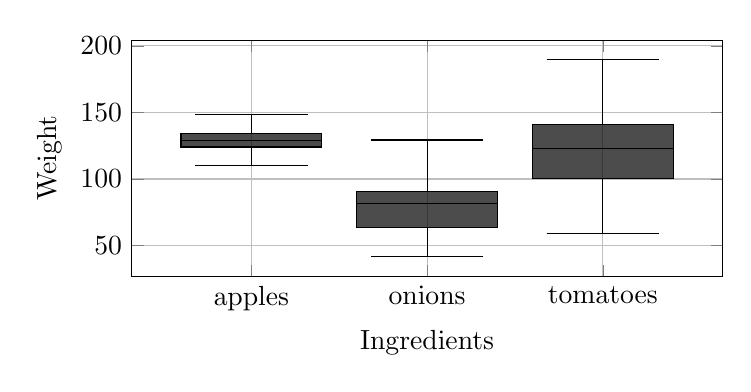
\begin{tikzpicture}
        \begin{axis}[
            ylabel=Weight,
            xlabel=Ingredients,
            xtick={ 1, 2, 3 },
            xticklabels={ apples, onions, tomatoes },
            width=7.5cm,
            height=3cm,
            boxplot/draw direction = y,
            at={(0cm,0cm)},
            scale only axis,
            axis background/.style={fill=white},
            grid=both,
]
            \addplot[
            fill,
            fill opacity=0.7,
            boxplot prepared={
                median=128.73043708220285,
                upper quartile=134.05952052012063,
                lower quartile=123.99094329503548,
                upper whisker=148.52278184508938,
                lower whisker=110.12431085399108
                            },
        ] coordinates {};
            \addplot[
            fill,
            fill opacity=0.7,
            boxplot prepared={
                median=81.68214339893669,
                upper quartile=90.76340895325481,
                lower quartile=63.886789536848525,
                upper whisker=129.26484224970574,
                lower whisker=41.62457569401917
                            },
        ] coordinates {};
            \addplot[
            fill,
            fill opacity=0.7,
            boxplot prepared={
                median=122.93087226956357,
                upper quartile=141.13312343712607,
                lower quartile=100.33669378132858,
                upper whisker=189.43975700020525,
                lower whisker=59.24572240027179
                            },
        ] coordinates {};
        \end{axis}
    \end{tikzpicture}
    \caption{Caption of the boxplot.}
    \label{fig:Caption of the boxplot.}
\end{figure}


\subsection{Bar chart}

\subsubsection{Default}

\begin{figure}[ht]
    \centering
    \tikzstyle{every node}=[font=\footnotesize]
    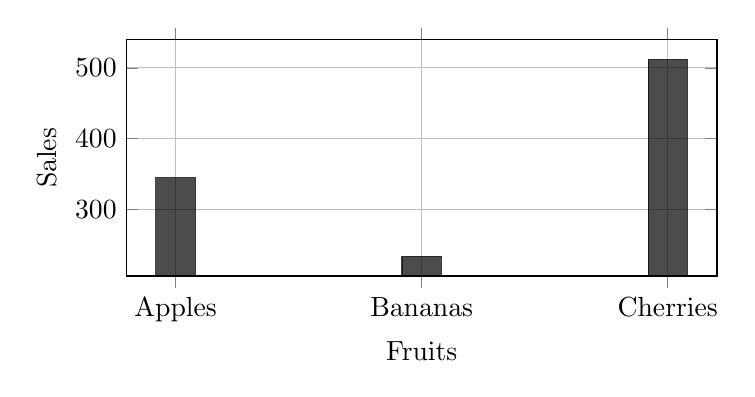
\begin{tikzpicture}
        \begin{axis}[
            ylabel=Sales,
            xlabel=Fruits,
            xticklabels={Apples,Bananas,Cherries},
            ybar,
            bar width=0.5cm,
            xtick=data,
            width=7.5cm,
            height=3cm,
            at={(0cm,0cm)},
            scale only axis,
            axis background/.style={fill=white},
            grid=both,
            legend columns = 1,
            legend style={at={(1,1.05)}, legend cell align=left, align=left, draw=white!15!black, mark options={draw=none}, anchor=south east},
        ]

        \addplot[fill=black!70!black,opacity=0.7]  
        coordinates {(1,345) (2,234) (3,512)};

        \end{axis}
    \end{tikzpicture}
    \caption{Caption of the default barchart.}
    \label{fig:Caption of the default barchart.}
\end{figure}


\newpage
\subsubsection{Multiple}

\begin{figure}[ht]
\centering
\tikzstyle{every node}=[font=\footnotesize]
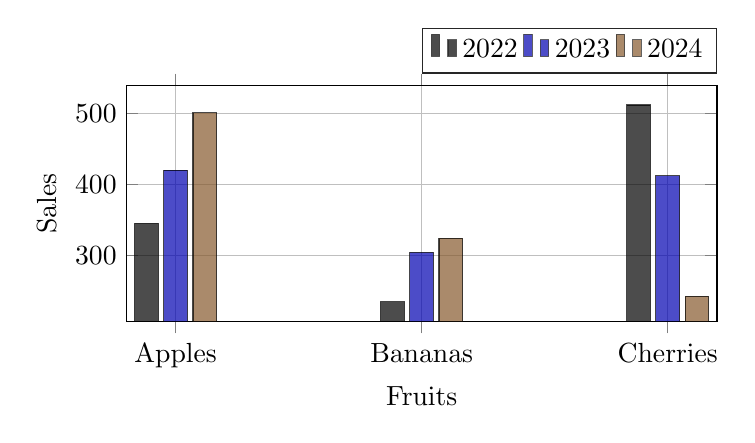
\begin{tikzpicture}
    \begin{axis}[
            ylabel=Sales,
            xlabel=Fruits,
            xtick={ 0, 1, 2 },
            xticklabels={ Apples, Bananas, Cherries },
            ybar,
            bar width=0.3cm,
            xtick=data,
            width=7.5cm,
            height=3cm,
            at={(0cm,0cm)},
            scale only axis,
            axis background/.style={fill=white},
            grid=both,
            legend columns = 3,
            legend style={at={(1,1.05)}, legend cell align=left, align=left, draw=white!15!black, mark options={draw=none}, anchor=south east},
    ]
        \addplot[fill=black!70!black,opacity=0.7]
            coordinates {(1,345) (2,234) (3,512)};
        \addlegendentry{2022};

        \addplot[fill=blue!70!black,opacity=0.7]
            coordinates {(1,420) (2,304) (3,412)};
        \addlegendentry{2023};

        \addplot[fill=brown!70!black,opacity=0.7]
            coordinates {(1,501) (2,324) (3,242)};
        \addlegendentry{2024};


    \end{axis}
\end{tikzpicture}
    \caption{Caption of the barchart.}
    \label{fig:Caption of the barchart.}
\end{figure}


\subsubsection{Stacked}

\begin{figure}[ht]
\centering
\tikzstyle{every node}=[font=\footnotesize]
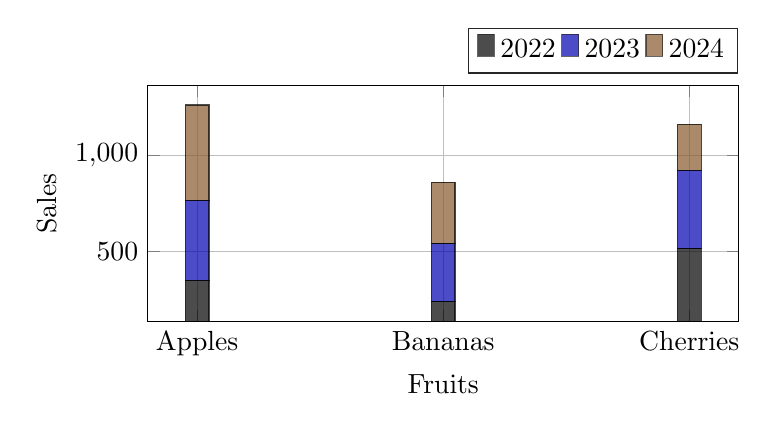
\begin{tikzpicture}
    \begin{axis}[
            ylabel=Sales,
            xlabel=Fruits,
            xtick={ 0, 1, 2 },
            xticklabels={ Apples, Bananas, Cherries },
            ybar stacked,
            bar width=0.3cm,
            xtick=data,
            width=7.5cm,
            height=3cm,
            at={(0cm,0cm)},
            scale only axis,
            axis background/.style={fill=white},
            grid=both,
            legend columns = 3,
            legend style={at={(1,1.05)}, legend cell align=left, align=left, draw=white!15!black, mark options={draw=none}, anchor=south east},
    ]
        \addplot[fill=black!70!black,opacity=0.7]
            coordinates {(1,345) (2,234) (3,512)};
        \addlegendentry{2022};

        \addplot[fill=blue!70!black,opacity=0.7]
            coordinates {(1,420) (2,304) (3,412)};
        \addlegendentry{2023};

        \addplot[fill=brown!70!black,opacity=0.7]
            coordinates {(1,501) (2,324) (3,242)};
        \addlegendentry{2024};


    \end{axis}
\end{tikzpicture}
    \caption{Caption of the barchart.}
    \label{fig:Caption of the barchart.}
\end{figure}



\end{document}
